\chapter{Cubesat-und Missionsdesign}
		\section{QuSAD}
			\subsection{Einführung in die Software}
Die Software QuSAD (SQL-Based CubeSat Analyse and Design Tool) besteht aus einem SQL-Segment und einem MatLab Segment. Die SQL-Datenbank ist die Haupteingabequelle für das Entwerfen eines CubeSats und kategorisiert die CubeSat-Komponenten. Durch die wissenschaftliche Version können die COTS-Komponenten mit vordefinierten Parametern eingepflegt werden. Des Weiteren können auch individuelle Komponenten mit veränderbaren Parametern mittels der praxis Version hinzugefügt werden. Für das Abrufen der Komponententabelle aus der SQL-Datenbank wird MatLab verwendet. Dies wird durch mehrere grafische Benutzeroberflächen (GUI) realisiert und ermöglicht dem Benutzer eigene Satellitenzusammenstellungen. Neben dem CubeSat Design können Budget Analysen von Masse, Volumen, Energie, Preis und Verlinkung durch zur Verfügung stehenden Werkzeuge erstellt werden, um folglich eine Optimierung des Entwurfs zu ermöglichen [Literatur]. Für ein vertieftes Verständnis der Software wird auf das QuSAD-Handbuch verwiesen [Literatur]. Das Anwendungsspektrum von QuSAD umfasst das erstellen eines Satelliten, sowie eine Bereitstellung einer Datenbank von Subsystemen für wissenschaftliche und auch lehrende Aspekte. Lehrende Aspekte umfassen den Einsatz der praktischen Version an Universitäten zur Unterstützung und Visualisierung [Literatur]. 

		\section{CubeSat- Designanalyse}
				\subsection{Angenommenes Design}
						Hier die Varainte von Max nehmen und kurz beschreiben
				\subsection{Triebwerkskonstelation}
				Hier alternative Triebwerkskonstellationen bzw. Anpassungen des Gesamtdesigns (wenn nötig) vorschlagen
								\textbf{Triebwerskonstellation 1}\\
								\textbf{Triebwerskonstellation 2}\\
								\textbf{Triebwerskonstellation 3}\\
								 etc.
				\subsection{Budgetplanung}
				
						\subsubsection{Massenbudget}
								
										\begin{figure}[h]
											\centering
												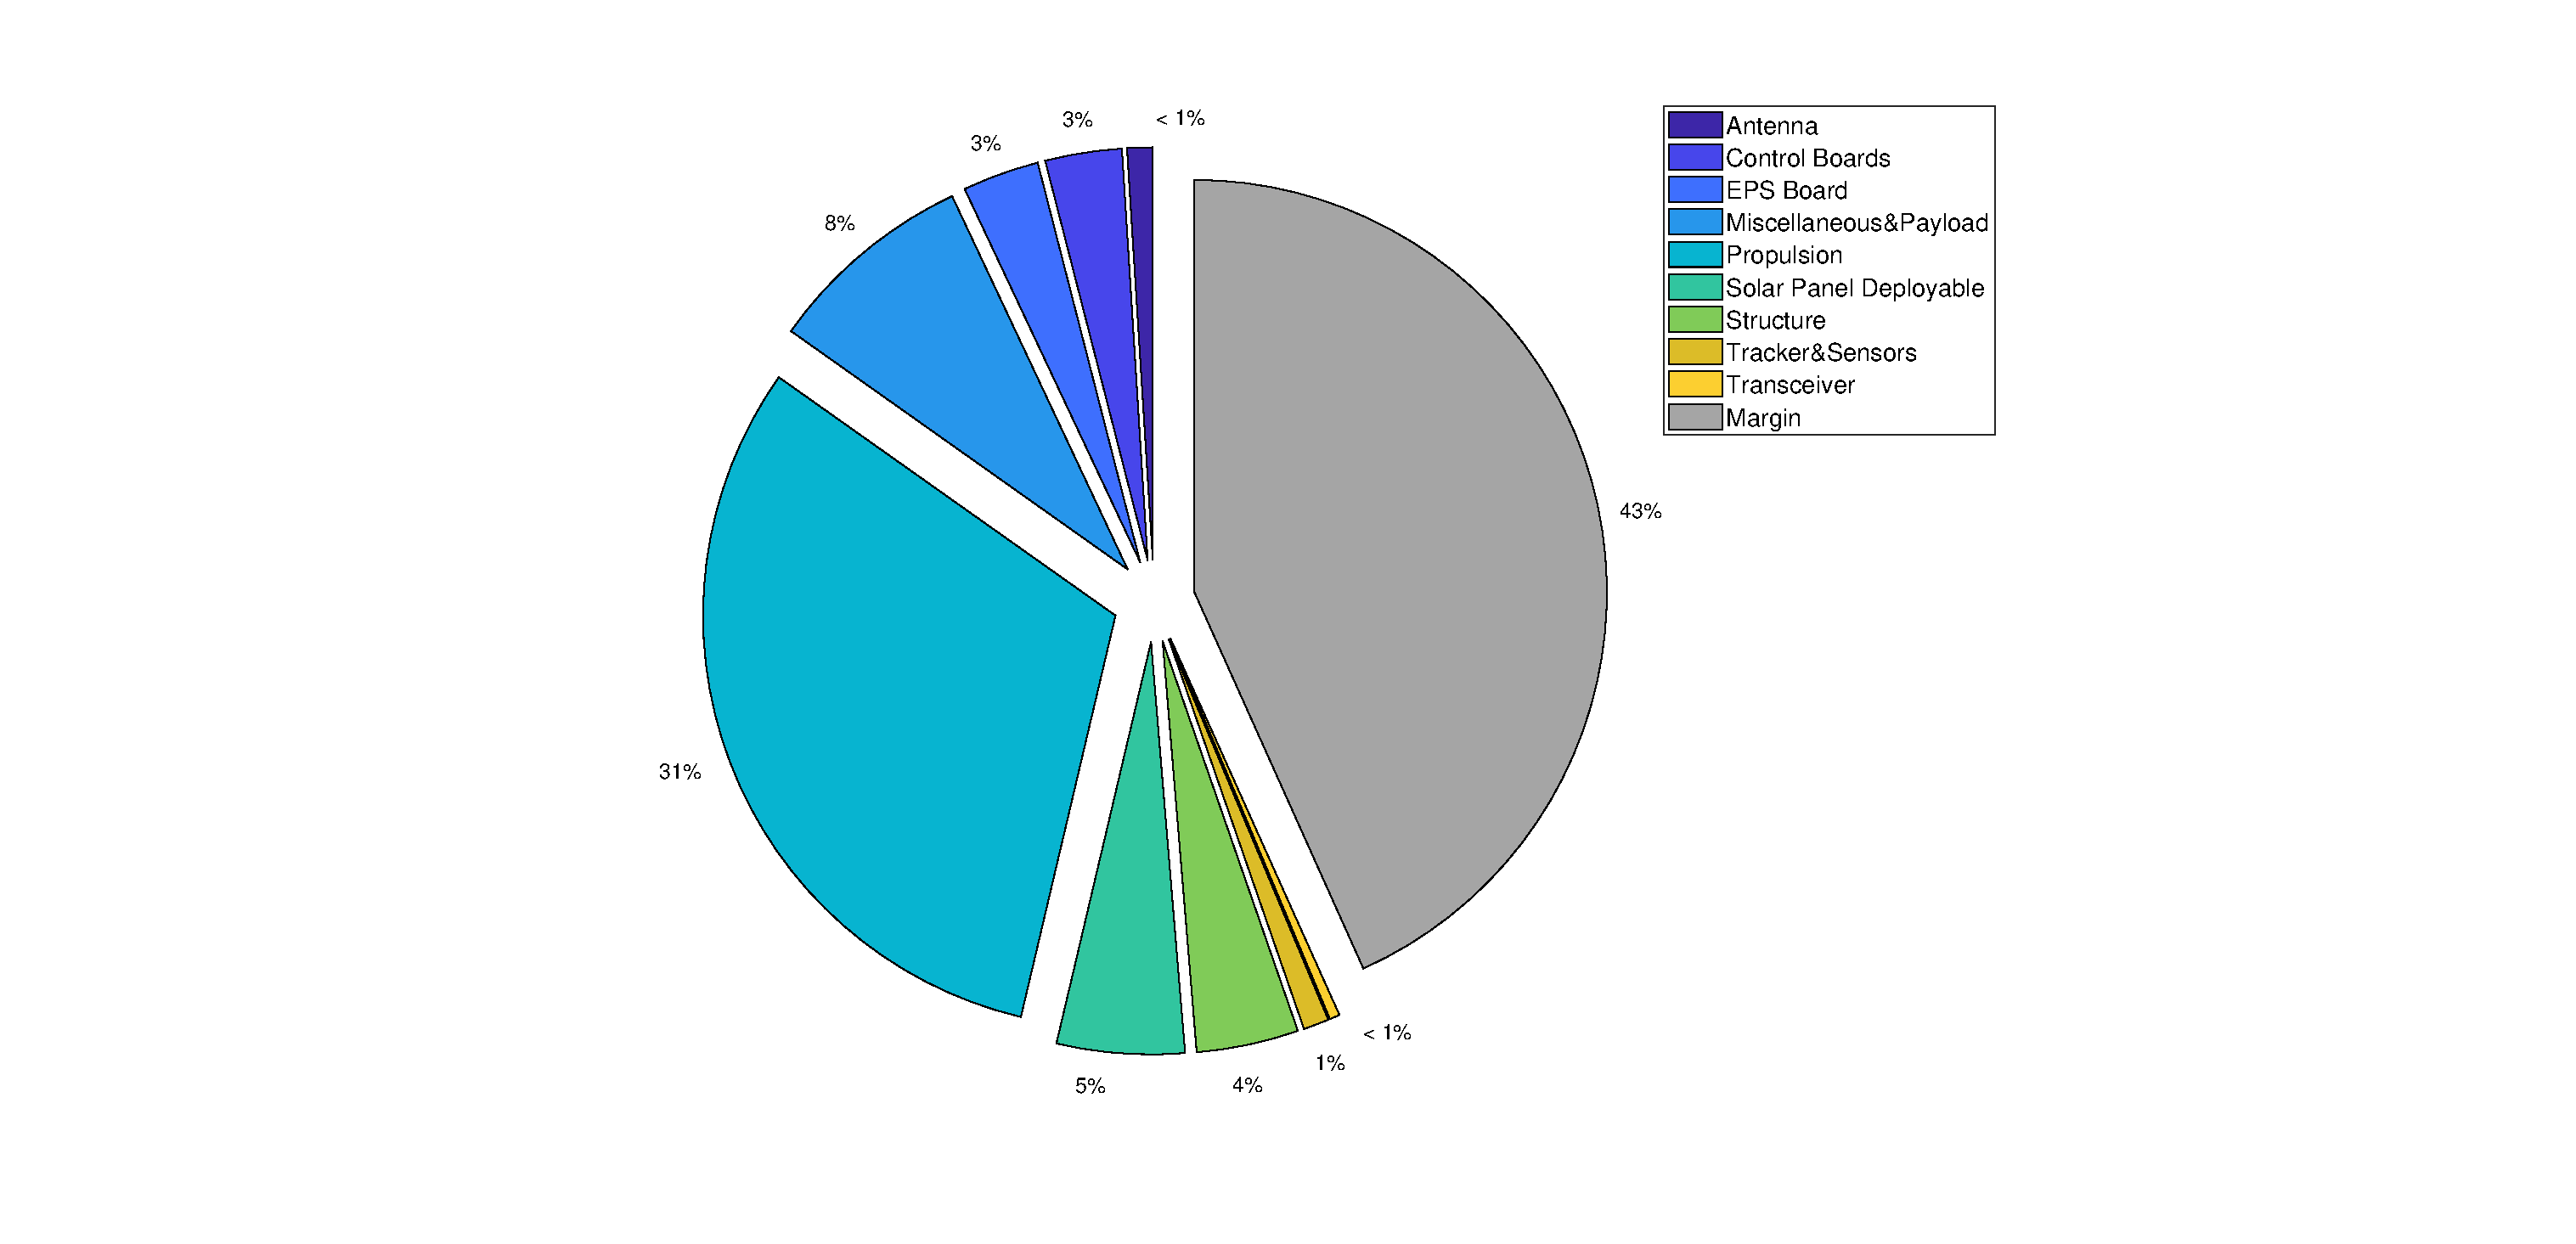
\includegraphics[width=1.00\textwidth]{masse}
											\caption{Massen Budget mittels QuSAD erstellt}
											\label{fig:masse}
										\end{figure}
										
						\subsubsection{Volumenbudget}
								
										\begin{figure}[h]
											\centering
												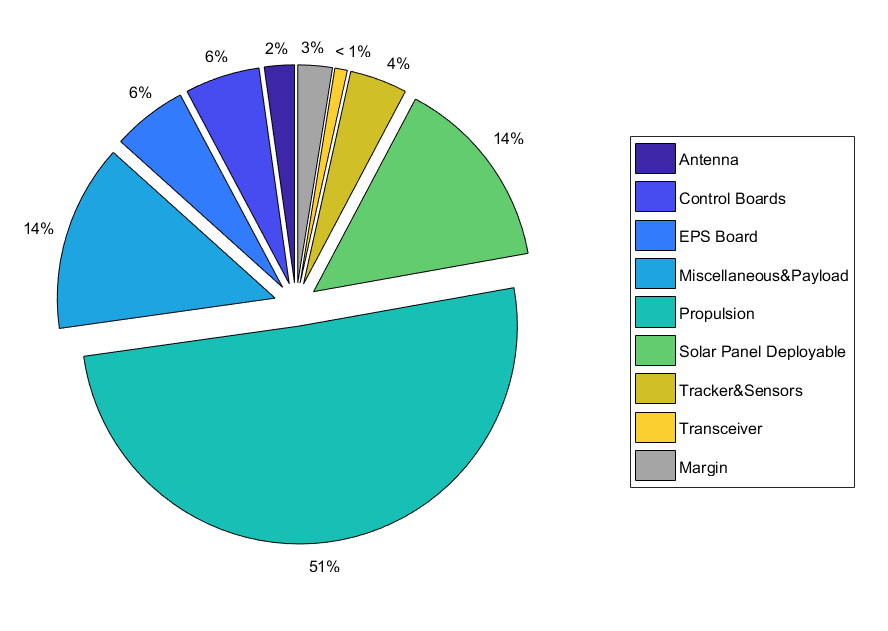
\includegraphics[width=1.00\textwidth]{volume}
											\caption{Volumen Budget mittels QuSAD erstellt }
											\label{fig:volume}
										\end{figure}
								
						\subsubsection{Leistungsbudget}
						\subsubsection{Preisbudget}
				
				\subsection{Konfigurationsvergleich}
		Budgets nur Vergleichen (kein GMAT) \\
		Datenbank soll möglichst nicht nur um die einzelnen Kompenenten erweitert werden (ruhig auch andere Komponenete aus der Excel Tabelle in die Datenbank aufnehmen)
		
		\section{	Ausgewähltes Missionsdesign}
		Kurze Beschreibung uas Max's Arbeit
				
